% XCircuit output "DUT.tex" for LaTeX input from DUT.ps
\def\putbox#1#2#3#4{\makebox[0in][l]{\makebox[#1][l]{}\raisebox{\baselineskip}[0in][0in]{\raisebox{#2}[0in][0in]{\scalebox{#3}{#4}}}}}
\def\rightbox#1{\makebox[0in][r]{#1}}
\def\centbox#1{\makebox[0in]{#1}}
\def\topbox#1{\raisebox{-0.60\baselineskip}[0in][0in]{#1}}
\def\midbox#1{\raisebox{-0.20\baselineskip}[0in][0in]{#1}}
   \scalebox{1}{
   \normalsize
   \parbox{6.66667in}{
   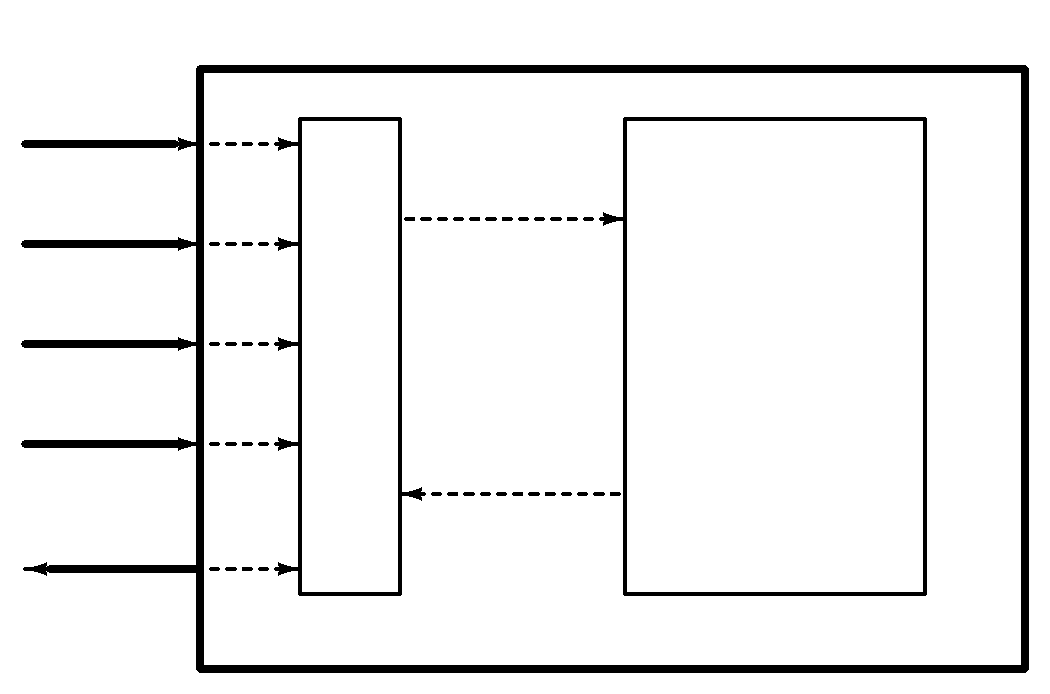
\includegraphics[scale=0.75]{DUT.eps}\\
   % translate x=1024 y=352 scale 0.38
   \putbox{3.59in}{1.56in}{1.20}{DUT}%
   \putbox{2.19in}{2.46in}{1.20}{dut\_in}%
   \putbox{2.19in}{0.66in}{1.20}{dut\_out}%
   \putbox{0.35in}{2.72in}{1.20}{TDI}%
   \putbox{0.27in}{2.22in}{1.20}{TCLK}%
   \putbox{0.31in}{1.73in}{1.20}{TMS}%
   \putbox{0.22in}{1.22in}{1.20}{TRST}%
   \putbox{0.31in}{0.6in}{1.20}{TDO}%
   \putbox{1.58in}{1.16in}{1.20}{\rotatebox{-270}{Scan Chain}}%
   \putbox{3.94in}{3.12in}{1.20}{mySystem}%
   } % close 'parbox'
   } % close 'scalebox'
   \vspace{-\baselineskip} % this is not necessary, but looks better
